\chapter*{Motivación}\label{sec:motivation}
\addcontentsline{toc}{chapter}{Motivación}

\section{Introducción}

La necesidad de comprender el proceso de aprendizaje y de personalizar la enseñanza para realizar una mejor adaptación a las necesidades del individuo ha motivado la \emph{Analítica de Aprendizaje} o \emph{Learning Analytics} \cite{Elias:LearningAnalytics}, disciplina que consiste en la recogida de datos de un entorno de aprendizaje y el análisis de los mismos cuyo objetivo es asistir en el proceso de aprendizaje del alumnado.

Además, el uso de laboratorios virtuales y remotos en la enseñanza está en auge. Entre muchas de sus ventajas tenemos una mayor privacidad para el alumnado, accesos planificados a los mismos o soporte para reportar la actividad de los alumnos y la calificación de los mismos.

En este trabajo fin de grado se usarán datos de siete cursos académicos obtenidos en el laboratorio virtual para sistemas multiagente de la asignatura del cuarto curso académico Desarrollo Basado en Agentes del grado de Ingeniería Informática de la Universidad de Granada (España).

El laboratorio virtual diseñado para la asignatura recoge el trabajo diario de los alumnos almacenando las interacciones entre los diferentes agentes y obteniendo así un extenso dataset que nos proporciona una base sólida para el uso de diversas analíticas de aprendizaje.

Así pues, se empleará un enfoque \emph{``data-driven''} o \emph{impulsado por datos}, tomando decisiones estratégicas basándose en el análisis de los datos y en la interpretación de los mismos.

Adicionalmente, este proyecto ha inspirado la presentación del artículo \emph{``In heaven as on earth: The performance of students is as good as it is the digraph that describes their behavior''} \cite{SIIE23} al \emph{XXV International Symposium on Computers in Education (SIIE)}.

\section{Motivación}

La principal motivación de este trabajo fin de grado es, precisamente, el análisis de los procesos de aprendizaje que siguen los alumnos para que el profesorado pueda asistirles mejor durante su proceso de aprendizaje y mejorar así su rendimiento académico.

Detectar grupos con dificultades para superar sus tareas de laboratorio es primordial para que el profesor pueda ayudarles y, cuanto antes, mejor. En este caso, el uso de técnicas de minería de procesos, comúnmente asociadas a indicadores de rendimiento de los alumnos, para extraer su comportamiento de un laboratorio virtual y la utilización de aprendizaje automático supervisado para identificar estos comportamientos han demostrado ser las herramientas fundamentales para identificar el comportamiento de los alumnos y prever grupos en riesgo. Así pues, en este estudio se demuestra que los indicadores de rendimiento de los alumnos pueden ser muy útiles, tanto como su comportamiento, estrictamente desde un punto de vista topológico.

\section{Objetivos}

El principal objetivo de este proyecto es identificar patrones de comportamiento indicativos de la evolución de los alumnos y del progreso de su aprendizaje, detectando, en las fases más tempranas posibles, comportamientos que pudiesen ser anómalos o que pudiesen indicar problemas de aprendizaje. Es decir, se pretende revelar, mediante la utilización de técnicas de minería de procesos, las posibles estrategias de los alumnos para cumplir los distintos objetivos de la asignatura así como desvelar su forma de trabajo habitual.

\section{Estructura del Trabajo Fin de Grado}

Este trabajo fin de grado consta de seis partes, $16$ capítulos y otros elementos como la portada, la declaración de originalidad, la autorización para su ubicación en la biblioteca de la escuela, la autorización para su defensa, sendos resúmenes tanto en español como en inglés (con sus respectivas palabras clave), la sección de agradecimientos, el índice general así como de una bibliografía y un apéndice.

A continuación se expone un breve esquema general del contenido de las partes y capítulos de este trabajo fin de grado:

\begin{itemize}
\item \hyperref[sec:parteI]{Parte I}: Motivaciones.
\begin{itemize}
\item \hyperref[sec:motivation]{\emph{Motivación}}: Se trata de un capítulo inicial en el que se expone una introducción en el contexto del proyecto junto con las motivaciones existentes, los objetivos que se pretenden conseguir con la realización del mismo y la estructuración de la memoria.
\end{itemize}
\item \hyperref[sec:parteII]{Parte II}: Estado del arte.
\begin{itemize}
\item \hyperref[sec:chapterI]{Capítulo 1}: Planteamiento del problema. Describe el funcionamiento de la plataforma educativa que recoge los datos que se usarán en este trabajo fin de grado y la clase de tareas que se le platean al alumnado que hace uso de la misma. Igualmente, se presenta un ejemplo ficticio que refleja el tipo de información recogida de la actividad de los alumnos.
\item \hyperref[sec:chapterII]{Capítulo 2}: Introducción a la Minería de Procesos y trabajos previos. Introducción al concepto clave de minería de procesos en relación a los objetivos que se plantean en este proyecto. Adicionalmente, se realiza una breve presentación de los estudios en este área previos a este trabajo y se realiza una clasificación de los trabajos realizados en el campo de la Minería de Procesos.
\item \hyperref[sec:chapterIII]{Capítulo 3}: Minería de Procesos. Breve descripción de la suite de minería de procesos Disco \cite{gunther2012disco} y de su algoritmo subyacente (\emph{Fuzzy Miner} \cite{gunther2007fuzzy}). Igualmente, se muestran algunos diagramas extraídos con dicha herramienta y se exponen sus principales limitaciones.
\item \hyperref[sec:chapterV]{Capítulo 4}: Teoría de grafos. Definiciones básicas relativas a la teoría de grafos entre las que se encuentra el concepto de \emph{Grafo Dirigido Acíclico}, concepto clave en el desarrollo de este trabajo. Además, se incluye la exposición y demostración del Teorema de Kirchhoff, generalización de la fórmula de Cayley que será de gran utilidad en el cálculo del número de árboles de expansión de grafos conexos. El capítulo finaliza con la presentación de algunas medidas de propósito general que se usarán para realizar una clasificación de los distintos grupos de prácticas.
\end{itemize}
\item \hyperref[sec:parteIV]{Parte III}: Planificación del proyecto.
\begin{itemize}
\item \hyperref[chapter:objetivos]{Capítulo 5}: Etapas del proyecto: división en objetivos. Se describen las iteraciones en las que se divide el proyecto siguiendo la metodología \emph{Scrum}.
\item \hyperref[chapter:sprints]{Capítulo 6}: Etapas del proyecto: división en sprints y seguimiento de los mismos. Se muestra la organización temporal del proyecto y el seguimiento del mismo mediante \emph{burndown charts}.
\end{itemize}
\item \hyperref[sec:parteIII]{Parte IV}: Análisis descriptivo.
\begin{itemize}
\item \hyperref[sec:chapterVI]{Capítulo 7}: Los registros existentes.  Incluye una descripción de los registros existentes en el servidor. Se muestra el número de grupos estudiados cada año, el periodo de tiempo analizado cada año y el conjunto de problemas analizados cada año, estudiando la dificultad de los mismos. Por último, se realiza un análisis de la actividad registrada en el servidor.
\item \hyperref[sec:chapterVII]{Capítulo 8}: Hipótesis de estudio. Exposición de las principales métricas de calidad definidas sobre los registros de actividad de los alumnos que podrían permitir discernir qué grupos presentan una mayor dificultad para resolver los problemas de prácticas propuestos. Se realiza una subdivisión de las mismas en continuas y a posteriori.
\item \hyperref[chapter:rendimiento]{Capítulo 9}: Rendimiento observado de los alumnos. Descripción detallada y estudio estadístico de las medidas de rendimiento de los alumnos clásicas. Se estudiarán las variaciones de las distintas variables a lo largo de los años y la normalidad de las mismas. El objetivo de este capítulo es la familiarización del lector con algunas de las métricas de calidad que serán determinantes en la predicción de grupos en riesgo.
\item \hyperref[sec:chapterIV]{Capítulo 10}: Implementación de la herramienta de Minería de Procesos \emph{Graph Miner}. Breve introducción a la manera en la que se representarán los grupos de prácticas en la herramienta de minería de procesos de creación propia \emph{Graph Miner}: la matriz característica de un grupo. Finalmente, se muestran los distintos gráficos que pueden obtenerse a partir de esta nueva herramienta.
\end{itemize}
\item \hyperref[sec:parteV]{Parte V}: Resultados obtenidos.
\begin{itemize}
\item \hyperref[chapter:correlations]{Capítulo 11}: Análisis de las correlaciones entre las distintas métricas. Análisis de la correlación existente entre las métricas clásicas para cuantificar el rendimiento de los alumnos y la nota obtenida por los mismos. Además, se estudiarán las correlaciones entre las medidas de complejidad (características topológicas de los grafos que representan el proceso de resolución de los problemas) y la nota alcanzada por los alumnos al final de la práctica.
\item \hyperref[sec:chapterXII]{Capítulo 12}: Perfiles de estudiantes según su rendimiento. Aplicación de técnicas de clustering para agrupar a los alumnos en diferentes intervalos de calificaciones empleando diferentes métricas (medidas clásicas de rendimiento y topológicas).
%\item \hyperref[sec:diferencias]{Capítulo 13}: Capacidad de distinción de las métricas. Estudio de las diferentes métricas respecto a su capacidad de separación entre alumnos en riesgo de obtener peores resultados y los que no presentarán dificultades para superar los problemas propuestos.
\item \hyperref[sec:chapterXIII]{Capítulo 13}: Clasificación de los grupos de alumnos según su rendimiento. Utilización del clasificador estadístico C5.0 para generar un conjunto de reglas que se emplearán para poder decidir si el rendimiento de una determinada agrupación de estudiantes es más bajo de lo que debería. Además, se utilizará otro clasificador del mismo tipo para predecir el intervalo de notas en el que se encontraría un determinado grupo de alumnos.
\end{itemize}
\item \hyperref[sec:parteVI]{Parte VI}: Conclusiones y vías futuras.
\begin{itemize}
\item \hyperref[sec:chapterXIV]{Capítulo 14}: Conclusiones. Repaso de los logros alcanzados a lo largo del proyecto y recapitulación de la principal motivación del desarrollo de este trabajo.
\item \hyperref[sec:chapterXV]{Capítulo 15}: Vías futuras. Exposición de un conjunto de propuestas para ampliar el trabajo aquí realizado.
\end{itemize}
\end{itemize}

\section{Repositorio de GitHub}

Para el desarrollo de este proyecto se ha creado el repositorio de GitHub \href{https://github.com/maribel00/Analysis-of-processes}{Analysis of processes} (Figura \ref{fig:repositorio}) para almacenar tanto los archivos fuente como la documentación del mismo. En él también podemos encontrar el archivo \texttt{README.md} (Figura \ref{fig:README}) con la siguiente información:

\begin{figure}[H]
    \centering
    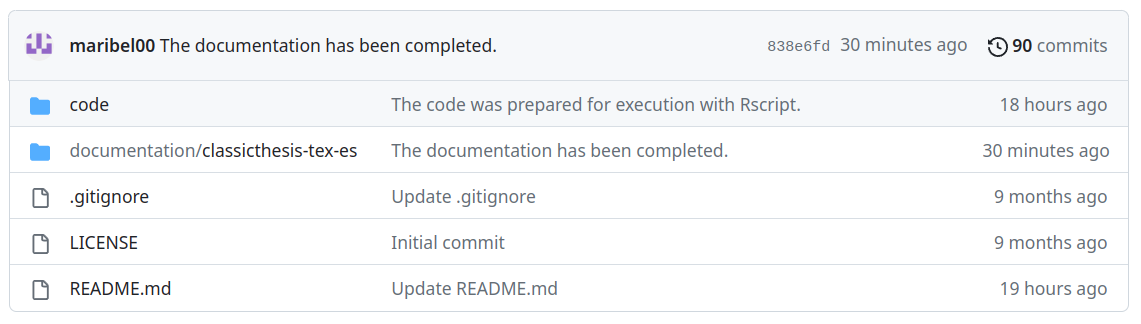
\includegraphics[width=0.80\textwidth]{motivación/estructura.png}
    \caption{Estructura del \href{https://github.com/maribel00/Analysis-of-processes}{repositorio de GitHub} creado para el desarrollo del proyecto.}
    \label{fig:repositorio}
\end{figure}

\begin{figure}[H]
    \centering
    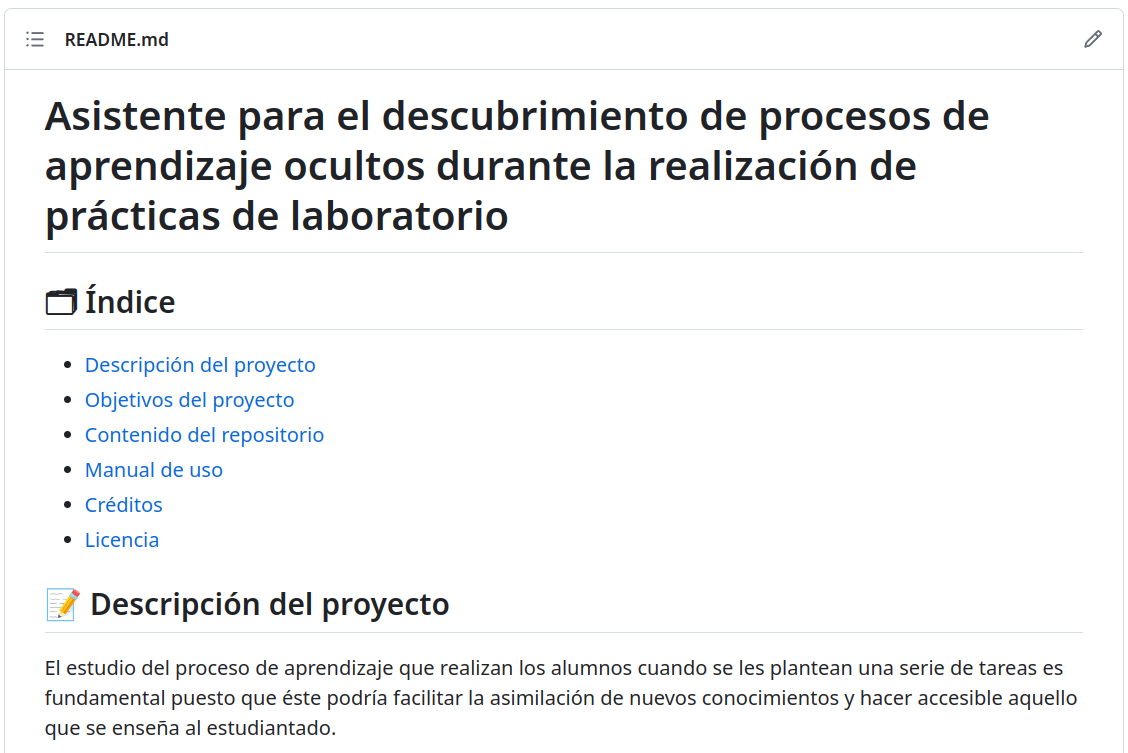
\includegraphics[width=0.80\textwidth]{motivación/README.png}
    \caption{Muestra del principio del archivo \texttt{README.md} incluido en el repositorio.}
    \label{fig:README}
\end{figure}

\begin{itemize}
\item Un índice para acceder cómodamente a todas las secciones del mismo.
\item La descripción del proyecto, en la que se realiza una introducción al contexto del proyecto y se destacan los logros conseguidos.
\item Una breve exposición del principal objetivo de este trabajo fin de grado.
\item Una descripción detallada del contenido del repositorio, incluyendo los datasets utilizados y destacando los archivos más relevantes para el proyecto.
\item El manual de uso para replicar los análisis estadísticos y experimentos que se exponen en esta memoria.
\item Una sección de créditos.
\item Una sección que enlaza con la licencia del proyecto.
\end{itemize}